\section{Sensorik}
\label{Sensorik_secd}
Die Aufgabe der verwendeten Sensorik liegt darin die Werte für $\varphi$, und $\dot{\varphi}$ zu bestimmen. Hierfür wurden zwei MPU6050 IC's verwendet. Diese verfügen jeweils über einen Beschleunigungssensor und Gyroskop, welche Werte für drei Achsen ausgeben. Der Tiefpass der Sensoren wird auf eine Grenzfrequenz von $44Hz$ eingestellt, da hier einerseits eine erste Glättung der Daten erfolgt, andererseits aber keine zu große Verzögerung ergibt, welche sich wiederum negativ auf die Regelung auswirken könnte. Die Position und Ausrichtung der Sensoren ist in \ref{Position_Sensoren_pic} dargestellt.

\begin{figure}[h]
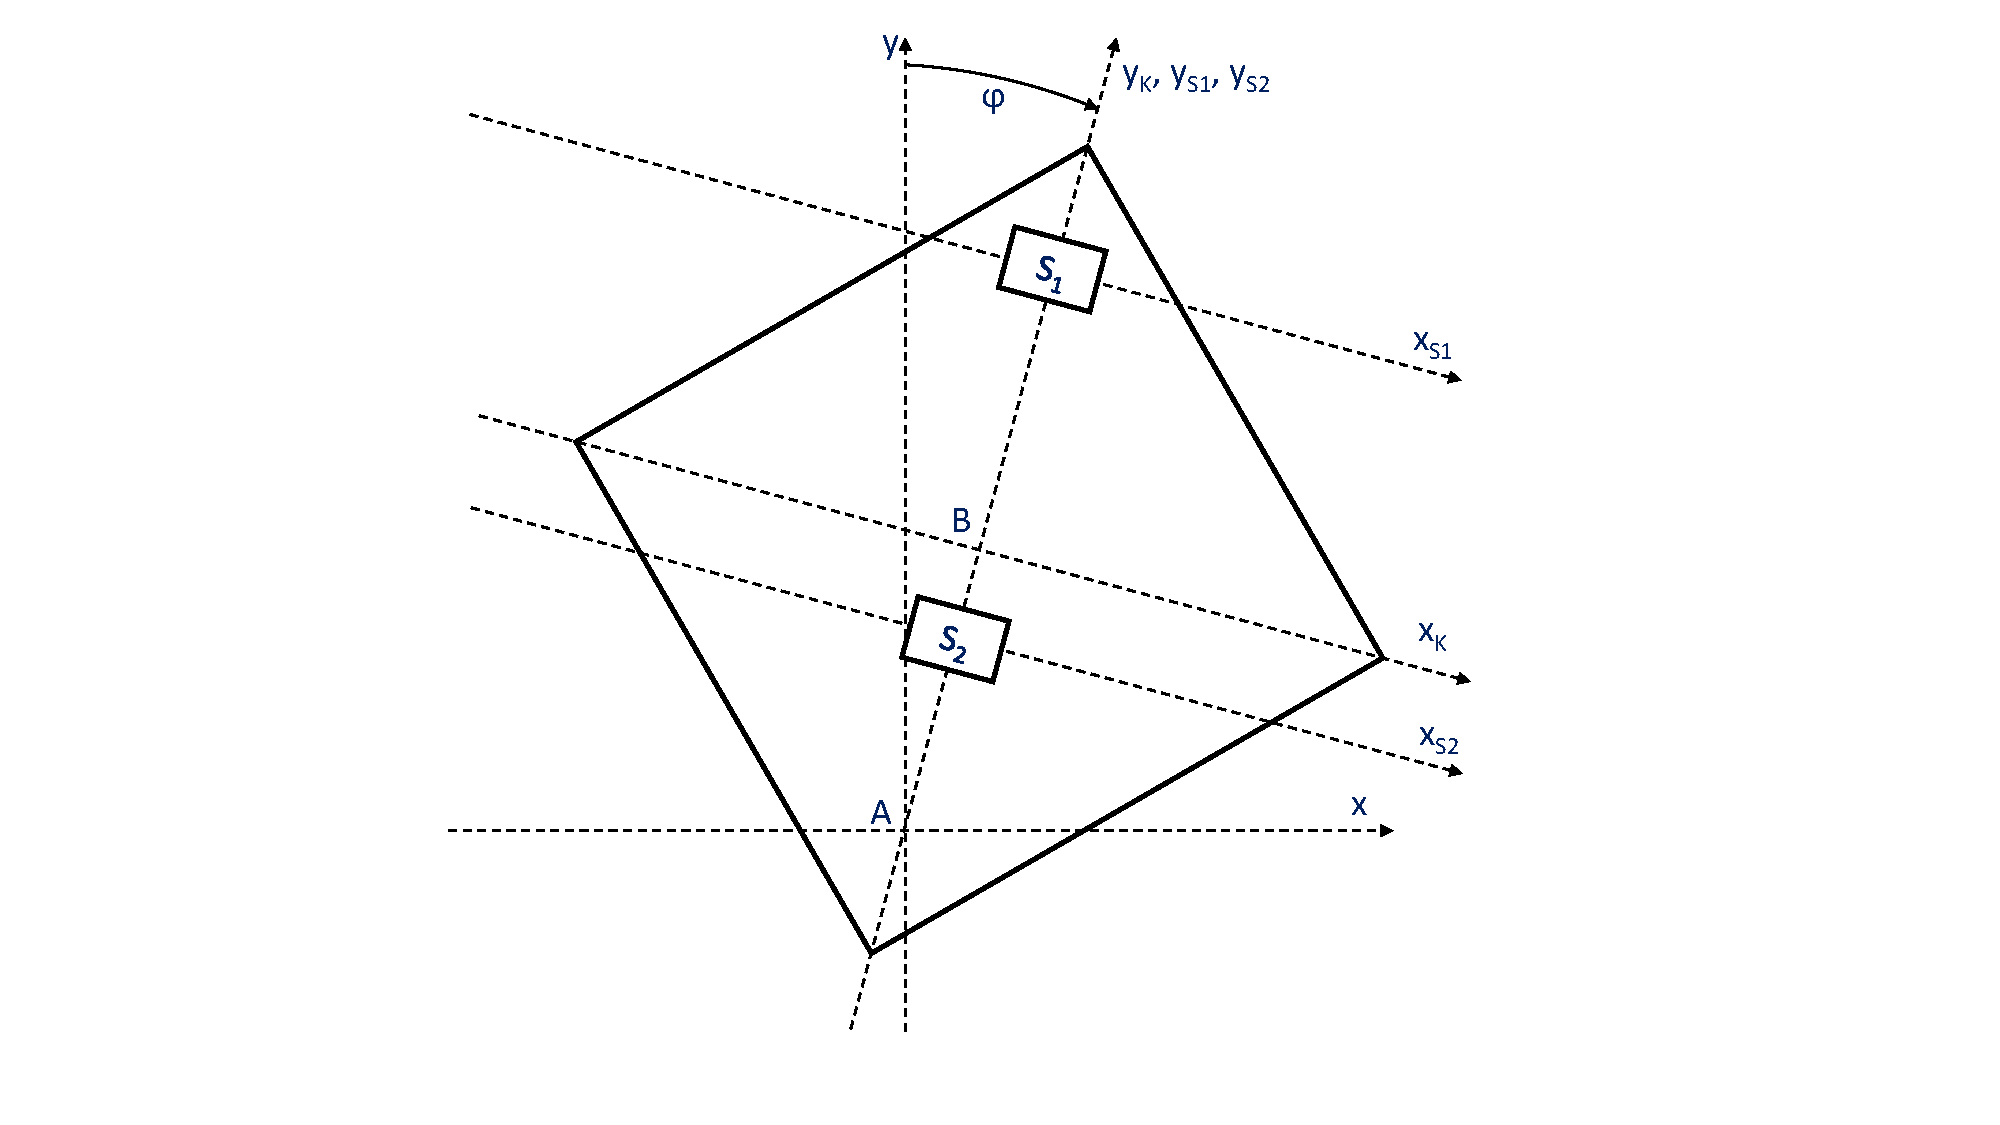
\includegraphics[width=\linewidth]{SensorZeichnung1D}
\caption{Position der Sensoren, Quelle: eigene Darstellung}

\label{Position_Sensoren_pic}
\end{figure}

\subsection{Winkelschätzung}
Die Sensoren keine Wege bzw. Winkel. Somit muss der Winkel $\varphi$ berechnet werden. Die gemessenen Sensorwerte hängen von $r_{S1}$ bzw. $r_{S2}$ ab, welche den Abstand zwischen den Sensoren und dem Drehpunkt $A$ beschreiben. Zusätzlich beeinflussen neben dem Winkel $\varphi$ auch dessen beiden Ableitungen $\dot{\varphi}$ und $\ddot{\varphi}$ die Sensorausgabe. Allerdings lassen sich aus den Beschleunigungswerten der beiden Sensoren nach \cite{Cubli1D} wie folgt der aktuelle Wert von $\varphi$ berechnen.

\begin{equation}
\ddot{S}_i = 
\begin{pmatrix}
\ddot{x}_i \\ \ddot{y}_i \\ \ddot{z}_i
\end{pmatrix} =
\begin{pmatrix}
r_{Si} \cdot \ddot{\varphi} + sin(\varphi) \cdot g \\
- r_{Si} \cdot \dot{\varphi}^2 - cos(\varphi) \cdot g \\
0
\end{pmatrix}
\hspace{35pt}
i \in [1;2]
\end{equation}

\begin{equation}
\alpha = \frac{r_{S1}}{r_{S2}}
\end{equation}

\begin{equation}
\ddot{x}_1 - \alpha \cdot \ddot{x}_2 = 
g(1 - \alpha)sin(\varphi)
\end{equation}
\begin{equation}
\ddot{y}_1 - \alpha \cdot \ddot{y}_2 = 
-g(1- \alpha)cos(\varphi)
\end{equation}

\begin{equation}
\frac{\ddot{x}_1 - \alpha \cdot \ddot{x}_2}{\ddot{y}_1 - \alpha \cdot \ddot{y}_2} = -tan(\varphi)
\end{equation}

\subsection{Kalibrierung und Justierung}
Die Sensoren geben die Beschleunigungs- und Geschwindigkeitswerte als 16 Bit Werte im Zweierkomplement aus. Diese Rohwerte müssen in die mit Hilfe eines Ausgleichspolynoms in die jeweilige SI-Einheit umgerechnet werden. 

\subsubsection{Umrechnung der Winkelgeschwindigkeiten}
In der Ruhelage werden 10000 Geschwindigkeitswerte der Sensoren aufgenommen. Über die Abweichung des Mittelwerts zu dem Sollwert ($\dot{\phi}=0$) wird die konstante Messabweichung ermittelt. Zusätzlich stellt der Hersteller einen Faktor zur Umrechnung der Roh- in SI-Werte. Daraus ergibt sich das folgende Polynom erster Ordnung zur Umrechnung der Gyroskopwerte in Winkelgeschwindigkeiten.


\subsubsection{Umrechnung der Beschleunigungswerte}
Um das Polynom zur Umrechnung der Beschleunigungswerte zu ermitteln werden sieben Messungen in den fixen Ausfallpositionen $\phi \in [-45, -30, -15, 0, 15, 30, 45]$ durchgeführt. Pro Position werden $m = 10000$ Messwerte aufgenommen. Da in der Ruhelage die Beschleunigung lediglich von dem aktuellen Ausfallwinkel abhängt ist der Sollwert für jede Position bekannt. Somit kann ein Polynom erster Ordnung approximiert werden um Mittelwerte der sieben Positionen in die entsprechenden Beschleunigungswerte umzurechnen.

%Bild mit Mittelwertvarlauf der Beschleunigungswerte x1, x2, y1, y2

\subsection{Auswertung der Radgeschwindigkeit $\dot{\psi}$}

\subsection{Filterung der Sensordaten}
In der Regel werden Sensoren von Störungen unterschiedlichster Art beeinflusst. Um diese Störungen zu minimieren werden in dem folgenden Abschnitt 
